%%!TEX encoding = UTF-8 Unicode

\documentclass[oneside]{ntuthesis}

\usepackage[utf8]{inputenc}

% Use biblatex instead of bibtex
\usepackage[backend=bibtex, style=ieee]{biblatex}
\addbibresource{bib/articles.bib}
\addbibresource{bib/books.bib}

\usepackage{mystyle}

%% Disable this package after finishing editing
\usepackage[disable]{todonotes}

% Type your personal information
%% Chinese
\setUniversityZH  {國立臺灣大學} 
\setCollegeZH     {電機資訊學院}
\setInstituteZH   {電機工程學研究所}
\setThesisTypeZH  {碩士論文}
\setTitleZH		  {網頁和手機程式自動化測試智能技術}
\setAuthorZH      {吳啟允}
\setAdvisorNameZH {王~凡}
\setAdvisorTitleZH{博士}
\setGradYearZH    {105} % The date is generated using \today
\setGradMonthZH   {7}   % You can un-comment and specify the date

%% English
\setUniversityEN  {National Taiwan University}
\setCollegeEN     {College of Electrical Engineering and Computer Science}
\setInstituteEN   {Graduate Institute of Electrical Engineering}
\setThesisTypeEN  {Master Thesis}
\setTitleEN		  {Intelligent Techniques for Automated Testing of Web and Mobile Applications}
\setAuthorEN      {Chi-Yun Wu}
\setAdvisorNameEN {Farn Wang}
\setAdvisorTitleEN{Ph.D.}
\setGradYearEN    {2015} % The date is generated using \today
\setGradMonthEN   {June} % You can un-comment and specify the date


\begin{document}
\begin{CJK*}{UTF8}{bkai}

\frontmatter
\maketitle   % Generate title page

%在這裡附圖(口試審定書)
% Dummy chapter for generating ToC
%\addcontentsline{toc}{chapter}{口試委員會審定書}
%
\includepdf[pages={1},pagecommand={}]{official/approvalZH-with-sign}
%\addcontentsline{toc}{chapter}{Oral Examination Approval Form}
%
\includepdf[pages={1},pagecommand={}]{official/approvalEN-with-sign}

\begin{onehalfspace}

\chapter{誌謝}

\setlength{\parindent}{2em}
首先最先感謝我的父母,
有了爸爸媽媽的支持與照顧,
在我低潮的時候鼓勵我勉勵我,
我才能順利完成我的學業。
我也要特別感謝指導教授王凡老師,
總是為我指引研究的方向。
老師教導我軟體測試的專業知識,
也教導我進行研究的方法和態度,
還提供許多機會讓我開廣見聞。
我還要感謝俊偉學長、庭芬學姊和汶宏學長,
因為他們的幫助,
我才能順利完成程式的開發,
對於程式的觀念也進步許多。
我也要感謝修博、宗儒和上誼,
這兩年一起修課,
在困難的時候一起扶持,
一起面對挑戰,
因為有你們的幫助,
我才能堅持完成這一切。
最後感謝所有實驗室的同學,
帶給我歡樂的研究室生活。
謝謝大家。








\end{onehalfspace}

\begin{onehalfspace}
\newcommand{\eng}[1]{\ \raisebox{1pt}{#1}}

\chapter{摘要}。

關鍵字:網頁測試、自動測試

\end{onehalfspace}

\begin{doublespace}

\chapter{Abstract}


Key words: software testing, test automation

\end{doublespace}

\begin{doublespace}
\tableofcontents
\listoffigures
\listoftables
\end{doublespace}


\mainmatter
\begin{doublespace}

\chapter{Introduction}\label{ch:introduction}

\section{Motivation}

Web Applications become more and more indispensable in our life.
People can easily get informations with the development of the Internet.
It becomes more convenient for people to search new knowledge, buy goods and chat with friends.
People spent lots of time on the Internet for working, studying, shopping, socialozong and playing.
As the result, more engineers tend to develop the applications on the Internet.
On the other hand, Mobile Applications is also a choice for software developer.
People can carry smart phone and enjoy the applications everywhere.
Although people can visit web applications by browser on the smart phone,
a special mobile application has a better performance.
Companies may develop the applications on both the Internet and the mobiles.
For instance, Google and Facebook.

In order to guarantee the performance and user experience of the applications,
the testing of the applications is required.
However, the current techniques of testing take lots of works and times.
Because the applications are complex and dynamic,
they have different reaction with different inputs.
Engineers need to write the test scripts case by case according to each functions.
they also need basic knowledge of software testing.
To reduce the work time of testing, the automated testing become essential for engineers.
But the challenge is it is too difficult to generate test case on black box testing.
Without the detailed information of functions,
We may not know how to make a test script.

%介紹software testing,其中又有web testing和mobile APP testing
%software變化大,需要測試確保功能正常,但製作testcase耗費時間人力
%auto testing的好處: 節省人力 black-box testing的好處:應用到所有APP
%建立一個auto testing ,開發者可減輕開發成本


\section{Purpose}

In this paper, we propose a technique to automatically generating traces on dynamic web applications.
The program named WebTraceCollector can collect the informations on web page and try to guess the suitable inputs.
We construct a inputs databank with some examples of inputs,
so the program will find a similar example as the input value of web page.
With the suggested input values,
the program can explore the website automatically and build the finite state machine to represent the website,
and generate the traces for testing.


In order to automatically evaluate traces collected from web and mobile applications,
we propose a teachnique to transform the traces into standard format.
We constrcut a label dictionary, which collects common sense of action and screen from applications,
so the traces can be expressed in a standard vector of labels.
Then, we use the method of machine learning to evaluate traces.
We use SVM to classify the traces into passed traces and failed traces.


%本篇建立了一個auto web testing的工具,和測試web,APP並驗證的framework
%framework將testcase取出symbolic label,train出所有APP可通用的model來evaluate all traces 


\section{Organization}

The rest of this paper is organized as follows.
Chapter 2 shows the related work, 
and we introduce the tool for generating mobile traces and the method used for evaluating in Chapter 3.
In Chapter 4, we propose a technique to generate traces on dynamic web applications.
Chapter 5 shows the framework to evaluate traces from the web and mobiles.
Then, the experiment results shown on the Chapte 6,
and the conclusion in Chapter 7.

%第二章 related work: 其他web,APP tesing, ex: selenium,crwaljax,splinter,Jmeter,UIautomata...
%第三章 preliminaries: machine learning,, test evaluation
%第四章
%第五章



\chapter{Related Works}\label{ch:related}

本篇測試的目標是web 和 Android APP,列出常見的testing 工具

\section{Web testing}

selenium,jmeter 需要先建立testcase 再重複測試

VeriWeb,CrawlJax可自動explore website,建立DOM tree,用DOM建state-based testing

\section{Android testing}

Ranorex,UIautomator 可測試Android APP

ADAutomation: behavior testing, GUI testing

\section{test evaluation}

test oracle use on software testing, finite state machine
% Barr [8]
metamorphic relations, 
Daikon


\chapter{Preliminaries}\label{ch:preliminaries}


\section{SpecElicitor}

SpecElicitor is a tool made by Yuan-Hong Lo, 
which can help user test Mobile Application with friendly GUI interface.

When user start using SpecElicitor,
each time user do an action on the Mobile Application, 
the tool will ask for labeling the action and the screen shown on the interface.
The interface is shown in Fig[].
By using SpecElicitor, we can choose the specified action at every step, label the meaning of the action,
and label the exception situation if it happen and stop the trace at any time we need.
The interface of the SpecElicitor is shown in Fig[\ref{SpecElicitorInterface}].


The traces made by SpecElicitor include automata, screenshots, XML files and labels.
The automata is a json file record every states and edges on the traces.
A state has a screenshot and a XML file dumped from the Mobile.
A edge records the action user did such as clicking element, typing text or exiting the Application.
The traces also record labels on every states and edges,
so we can recognize how many label we focus on happened on the trace.
An example trace of Recipe Application made by SpecElicitor is shown in Fig[\ref{SpecElicitorTraces}].

%Our LAb 建立了一個工具SpecElicitor
%使用者可以在GUI介面下一邊建立APP的trace, 同時標記該畫面/動作的label
%使用完後會產生含有 XML, 截圖, label的traces

\begin{figure}[h]
	\graphicspath{{pic/}}
	\begin{center}
		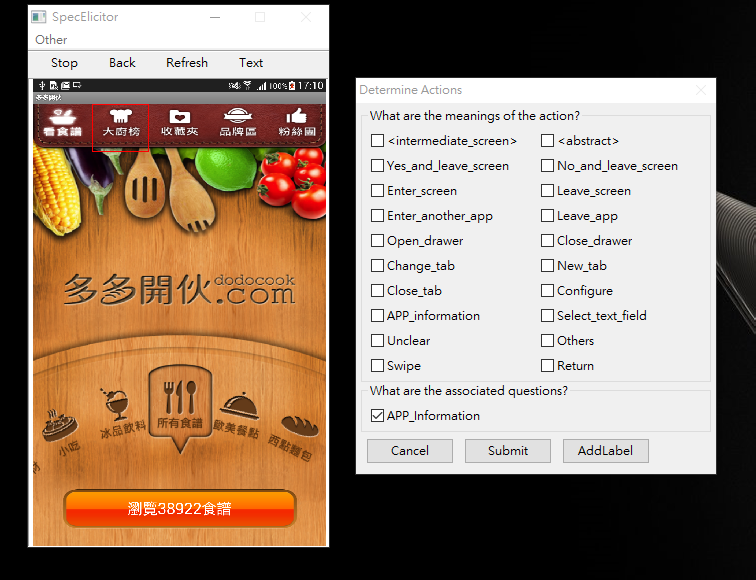
\includegraphics[width=0.8\textwidth]{SpecElicitorInterface.png}
		\caption{ The GUI interface of SpecElicitor.  }
		\label{SpecElicitorInterface}
	\end{center}
\end{figure}

\begin{figure}[h]
	\graphicspath{{pic/}}
	\begin{center}
		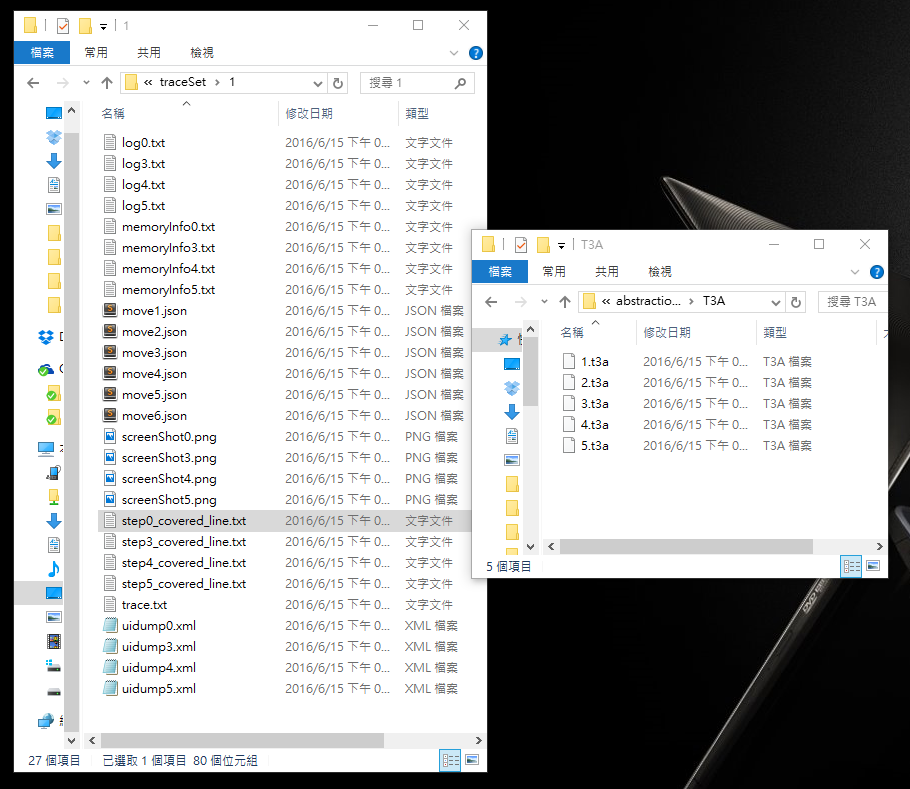
\includegraphics[width=0.8\textwidth]{SpecElicitorTraces.png}
		\caption{ An example of the traces.  }
		\label{SpecElicitorTraces}
	\end{center}
\end{figure}

\clearpage

\section{Common Sense Model}

將APP建立出state-base的automata,其中screen作為state,action作為edge

用統一的normalized terms來specific

our Lab建立一個TAAD的SpecElicitor,可產生label的trace


\section{Support Vector Machine}

SVM 在高維度 用largest margin來 seperate datas 

SVM可用來 cluster data

\chapter{WebTraceCollector}\label{ch:traceCollector}

In order to testing web applications,
we need collects a variety of test cases 
for finding the bugs, analyzing the reasons why the failure happen 
and ensuring the application can work successfully in any circumstances.
However, recording the behaviors on browser manually costs lots of time and work.
It is important to improve the efficiency of web testing by generating test traces automatically.
Thus, we need a tool that can automatically explore web applications and record the traces.

We make a tool named WebTraceCollector that will be introduced in this chapter for automatically generating traces of Websites.
WebTraceCollector is wrote on Python 3 and using Selenium as Library.
It can open a browser with selenium and explore the Website with the browser automatically.
Depending on the Document Object Model\cite{DOM} of the current web page,it will find the suitable clickable elements to click.
WebTraceCollector can also work fine on the dynamic websites with Ajax\cite{ajax} application,
and insert texts into every input text fields with the fitting data.

%為了測試APP和WEB,our lab使用了一些工具來產生traces
%this paper 用python 和 seleium為基底建立一個可以自動explore website的trace collector
%此工具用DOM tree來做state-base的finite state machine

\clearpage

\section{Framework}

There are several kinds of work,
such as taking snapshot, inserting values and deciding the next element to click, during the web testing.
To manage all works, WebTraceCollector collects all events by a list.
It also constructs a finite state machine to record every web page in the website 
and represent the link between web pages by the edges and states.
The framework of WebTraceCollector is shown in Fig \ref{collectorFramework}.

At the first step of testing, WebTraceCollector go to the target URL and start to recognize the first web page.
The web page will be converted into a state of a finite state machine.
In order to explore the website deeper,
the clickable elements and input fields should be identified and 
the next action event depending on the clickable elements will be added into the event list.
WebTraceCollector constantly get an event from the list
and implement a event at once until the list is empty.

After implementing an action, WebTraceCollector will check the status of the webpage.
If the web page changes, the new web page will be converted into a new state and saved in the automata.
Similarly, the clickable elements of new web page should be identified and 
the events of new clickables will be added into event list.

The algorithm of WebTraceCollector is shwon in algorithm \ref{AutomataOverview}.

\begin{algorithm}[htb]
	\begin{doublespace}		
		\KwIn{ URL, algo }
		Initial(URL)\;
		Current\_State $\gets$ Web\_Page\;
		Automata.add\_state( State )\;
				
		\While{ Event\_List $\neq$ Empty }
		{
			Event $\gets$ Event\_List.Get\_Event()\;
			Do\_Event( Event )\;
			Next\_State $\gets$ Web\_Page\;
			\If{ Next\_State $\neq$ Current\_State  }
			{
				Automata.add\_state( Next\_State )\;
				Event\_List.Add\_Event( Next\_State )\;
			}
			Current\_State $\gets$ Next\_State\;
		}		
	\end{doublespace}
	\caption{Overview}
	\label{algorithm:overview}
\end{algorithm} 

\begin{figure}[h]
\graphicspath{{pic/}}
\begin{center}
	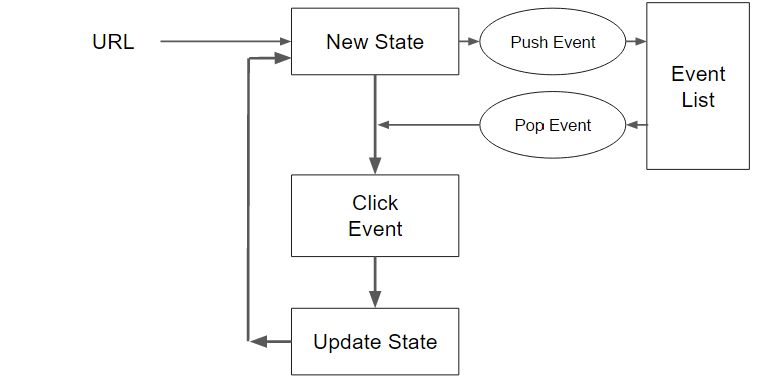
\includegraphics[width=0.8\textwidth]{collectorFramework.png}
\end{center}
\caption{The framework of WebTraceCollector. }
\label{collectorFramework}
\end{figure}

%此工具一邊使用selenium來操縱web browser,
%一邊建立state(DOM), edge(click ,inputs) 的automata
%此工具使用event list的形式,選擇一個algorithm,每次pop out一個待辦的event
%每次update:若是新的state,就將所有的clickables排入events,若是舊的state就無視

\clearpage

\section{Webpage identification}

WebTraceCollector record the current page of the browser into a state in the finite state machine.
In order to identify a web page,
we distinguish the web pages according to the DOM tree.
The DOM tree is the tree structure of the web elements.
However, we can not directly access the DOM tree of the web page by the browser,
the method to solve this problem is downloading the page source of web page by selenium 
and rebuild the DOM tree by the library BeautifulSoup\cite{BS4}.

After building the DOM tree, the elements in the web page are known.
The clickable elements are defined as <a> tag, <button> tag and <input> tag with button attribute. 
WebTraceCollector find all the clickable elements in the DOM tree
and convert them into event objects.
The events will be added into event list,
so the testing will continue to click these element later.

In some complex case, the website is not only work by the simple buttons 
but also javascript functions that have bind mouse listener on other elements.
It is almost impossible to guess which element have the javascript function,
becuase we only do black box testing of the web applications 
and we do not know how the web applications work 
for understanding the javascript code in the web page is too difficult.
Even so, most of the web applications still can tested by this method,
and automated testing still saves lots of human effort.

\clearpage

\section{Event}

During the testing, WebTraceCollector repeats getting an event from the event list 
and implements the action of the event until the event list is empty.
The procedure of event is shown in Fig \ref{ClickEvent}.
An event consists of action, state and depth.
The action implies which clickable element should be clicked.
The state implies where web page the element locates in.
The depth implies how deep this event is in the automata.
Every event has only one action, which means it only click one button at one time.
According to the DOM tree of the web page, the clicking action will insert the value into the input fields.

Before the event start, 
WebTraceCollector checks the current state on the browser.
Because if the current state is not equal to the state recorded on the event,
the wrong element will be clicked and the change of the state will be recorded and lead to wrong automata.
If the current state is not equal to the state on the event, 
it should change the web page to where the clickable element locates.
Most of the time, it can reached by trace back history from the browser.
But in the case of complex website ,it will be hard to retrun the correct web page.
In that case, the automata find the simple past from the initial state of wepsite to the target state,
and WebTraceCollector will go through the simple path to reach the target web page.

Once the arrive to the correct web page, WebTraceCollector will start to clicke the target element.
However, web pages not only have clickable elements,
the dynamic web pages also have input fields need to insert and 
lead to different reaction according to the value that user inserted.
To work fine on those dynamic websites that not only have buttons to click but also have other input fields,
WebTraceCollector needs to insert values into those elements when it implements the clicking action.
The input field elements are defined as <input> tag, <select> tag, <radio> tag and <checkbox> tag.
Because the Website may only accept certain words as input values likes, 
we can not just make random string to test the Website.
we construct a database to analysis the element and find the most suitable string.
The database has some example values of the common inputs we generalize from websites.
Considering the element's tag, id, name and other siblings tags,
WebTraceCollector will use the most similar string to the examples as the input value of the element.
The algorithm of implementing the action is shwon in algorithm[\ref{algorithm:action}].

\begin{algorithm}[htb]
	\begin{doublespace}		
		\KwIn{ action, state, depth }
		\If{ Current\_State $\neq$ state }
		{
			Back\_Track( state )\;
		}
		Clickable $\gets$ action.Get\_Clickable()\;
		Inputs, Selects, Radios, Checkboxes $\gets$ state.getFormElements()\;
		\ForEach{ Element in Inputs, Selects, Radios, Checkboxes }
		{
			Value $\gets$ Database.Find\_Value( Element )\;
			Set\_Value( Element, Value )\;
		}
		Click\_Clickable()\;		
	\end{doublespace}
	\caption{To implement the action}
	\label{algorithm:action}
\end{algorithm} 


\begin{figure}[h]
	\graphicspath{{pic/}}
	\begin{center}
		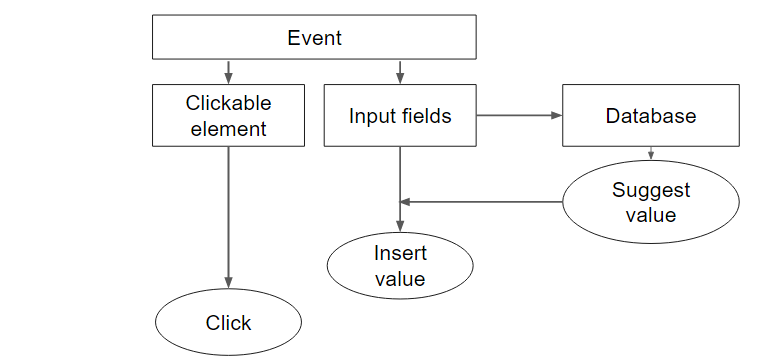
\includegraphics[width=0.8\textwidth]{ClickEvent.png}
	\end{center}
	\caption{The  procedure of click event. }
	\label{ClickEvent}
\end{figure}

%要執行click action時,會先對所有的input 填值,會連上database進行input,clickable的tag等feature的字串處理,找出推薦的適當的值填入

\clearpage

\section{Suggested value}

The problem of guessing the correct value of specific input field is very difficult.
Because we only implement the black box testing, it is hard to realize the meaning of the current web page
while unknowing the whole codes of the web applications.
The method we can use is analyzing the text of the element 
and trying to guess the meaning of the input element.

We constrcut a database which storing lots of example values of common input elements.
A partial of the database is shown in Table \ref{InputDatabase}.
Each data is an example value of a common feature 
and each feature has several normalized keywords.
For example, a feature email has keywords "email" and "信箱" and some exmple valuse like "Ann@gmail.com".
For a specific input element,
we analyze the element's tag name, id attribute, name attribute and text.
If the attributes of the elements similar to the keywords of a feature,
we will suggest that the feature is suitable to be the value of the input element.
Then, one of the examples randomly selected and insert into the input field.

While an event is implementing, WebTraceCollector not only choose the target clickable element
but also need to insert the suitable value into every input fields on the web page.
Those input fields' detailed infomation will analyzed with the database 
and the sugested value will generated by string analysis.


\begin{table}[ht]
	\begin{center}
		\begin{tabular}{ | l | l | l | l | }
			\hline
			Feature & value 1 & value 2 & value 3 \\ \hline
			email / 信箱 & Ann@hotmail.com.twn & Bob@gmail.comn & Cindy@yahooo.com \\ \hline
			name / 名字 & Ann & Bob & Cindy \\ \hline
			job / 職業 & studentn & engineern & officer \\ \hline
			gender / 性別 & man & woman & \\ \hline
			phone / 電話 & 0900123456n & 0987654321n & 0911001011 \\ \hline
			address / 地址 & \#12 abc street & 5 floor \#12 sun street & \# USA   \\
			                & Tainan Taiwan  &  Pintung Taiwa         & orange,2323 \\ \hline
			birth / 生日 & 2001/02/03 & 1999/04/03 & 1988/11/30 \\ \hline			
		\end{tabular}
		\caption{ Part of the input database. }
		\label{InputDatabase}
	\end{center}
\end{table}

\section{Normalization}

After the action, WebTraceCollector will check what happens on the browser 
by comparing the current state of the web page and other states in the automata.
The state objects have the information of DOM tree loading from the browser by Selenium.
If the DOM tree is same after click event, the clickable element will be regarded as ineffective and no edge and reaction will happen.
On the other hand, if the DOM tree changes, the clickable element will be regarded as effective link.
The clickable and the input values will made as a edge and added into automata.

However, there are some problems if we just regard the two DOM trees as strings and compare.
For example, there may be advertising applications, calenders, popularity numbers or catalogs shown on the website.
Each time user visits the website, the DOM tree of the website may be different.
To prevent recognizing a wrong state, we must preprocess the DOM tree.

The work of preprocessing is removing the elements that may confuse us and remain the elements we want to focus on.
We remove the tags that are unvisible on the web page, the javascripts code, the HEAD of the html and the css style.
We construct a class named normalizer, which can scan the DOM tree, find the target element and remove it.
For specific website, User can set the specific normalizer to normalize the DOM tree by his own style.
The examples of DOM tree and normalized DOM tree are shown in Fig[\ref{DOMvsNorDOM}].

%state用DOM比較,但有問題需要省略
%省略的方式有config

\begin{figure}[h]
	\graphicspath{{pic/}}
	\begin{center}
		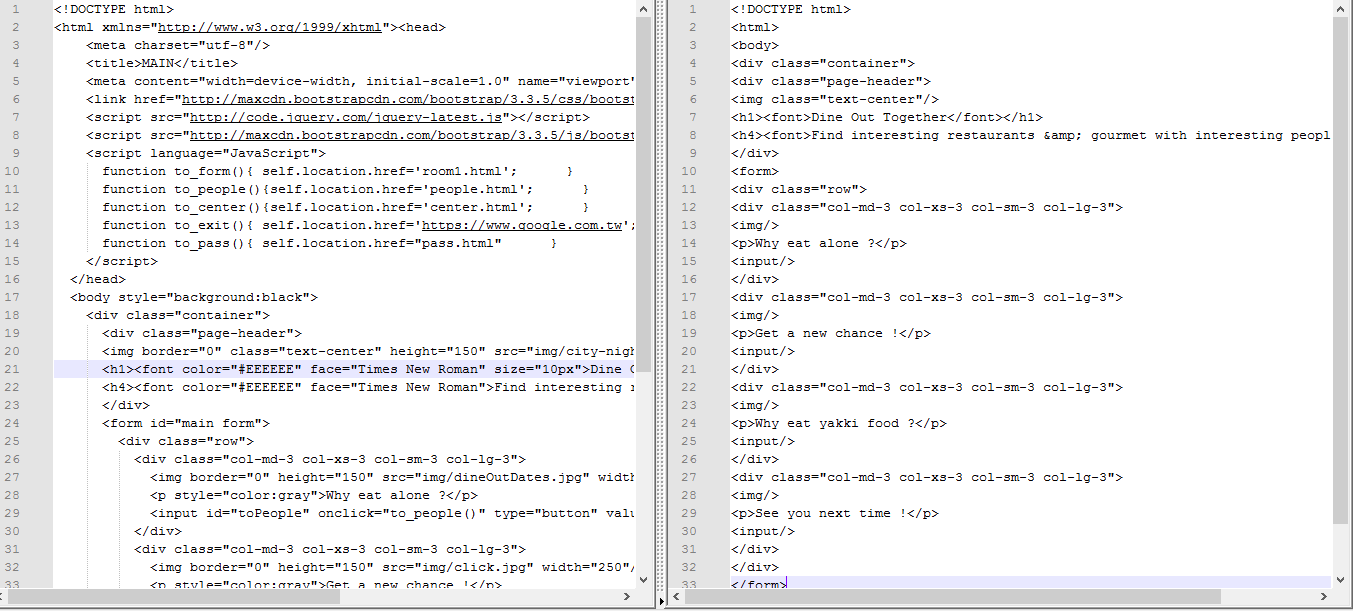
\includegraphics[width=0.8\textwidth]{DOMvsNorDOM.png}
	\end{center}
	\caption{An Example of DOM tree compare with Normalize DOM tree. }
	\label{DOMvsNorDOM}
\end{figure}

\clearpage

\section{Automata and traces}

We construct an finite state automata, which consists of states and edges, to represent the Website
with each state represent a web page and each edge represent the link from one web page to another.
The state is defined based on the DOM tree of the web page.
If the URL, DOM tree or any element on the web page changes, we will recognize that it goes to other state.
The edge records one state goes to another state by an action,
which clicks the specific clickable tag with values written in all form elements.

In order to view the automata clearly and help user to understand the automata easily,
WebTraceCollector generate a HTML file to show the graph of the automata.
In the html, every state represented by the snapshot of the web page,
and every edge between two states are represented by the arrows connected between the two states.
The example web page of automata is shown in Fig[\ref{AutomataOverview}].

As the test result, WebTraceCollector generates traces information in different types of files. 
There are JSON files of traces and automata, screenshots of every state, DOM tree and detail information of every state and a web page of overview automata.
Automata.json records all states, which have URL, ID, screenshot and DOM tree of the web page, and edges.
Traces.json records the states and edges with the order
The example of the test result is shown in Fig[\ref{TestResult}].

\clearpage

\begin{figure}[h]
	\graphicspath{{pic/}}
	\begin{center}
		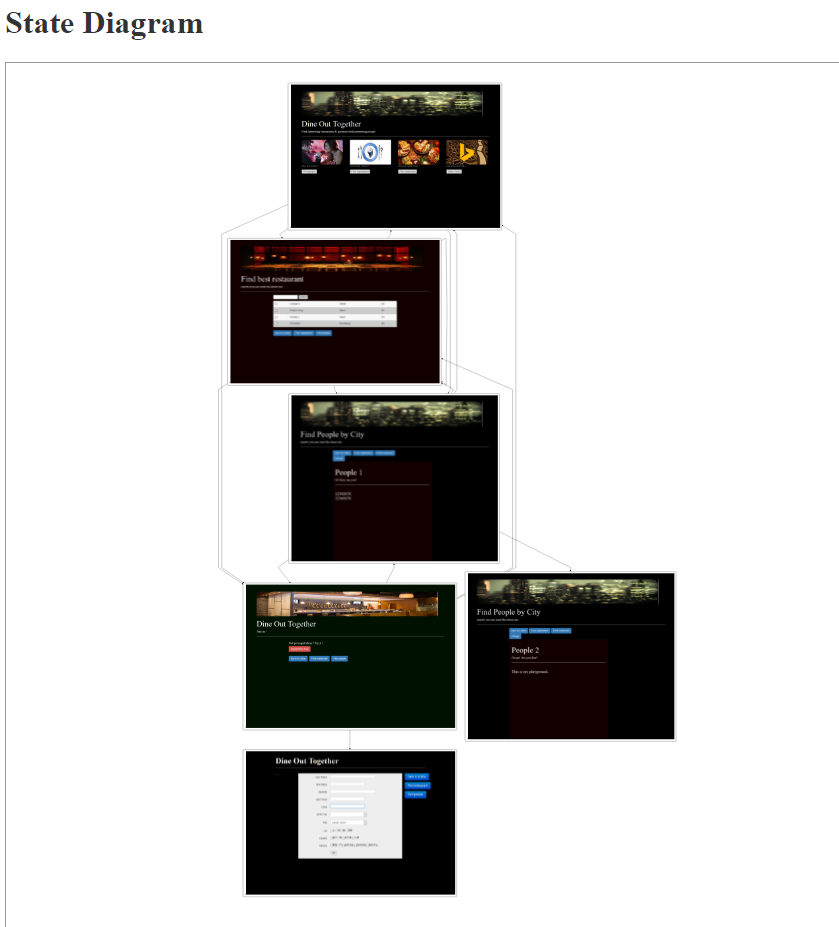
\includegraphics[width=0.6\textwidth]{automata_overview.png}
	\end{center}
	\caption{ Overview of the Automata. }
	\label{AutomataOverview}
\end{figure}

\begin{figure}[h]
	\graphicspath{{pic/}}
	\begin{center}
		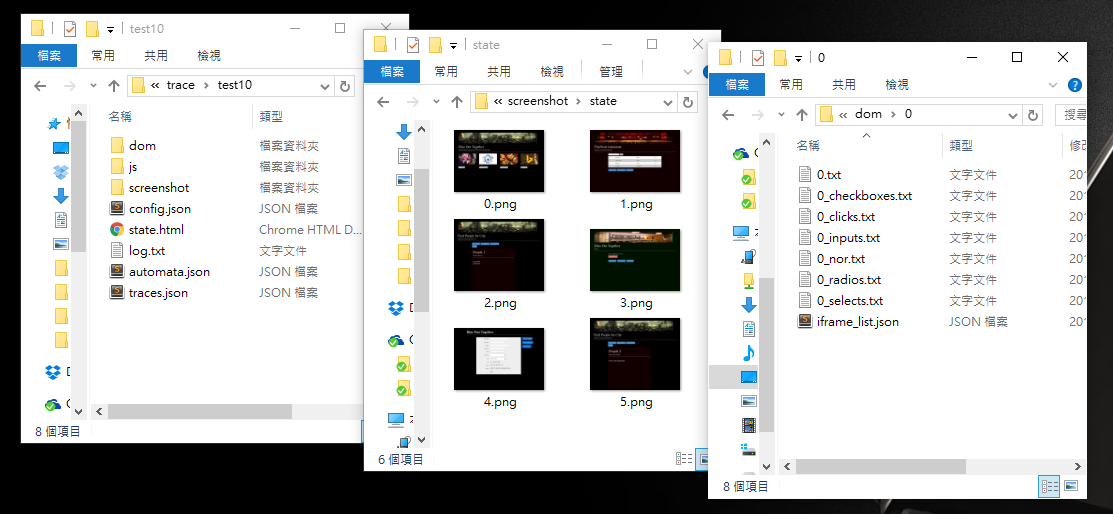
\includegraphics[width=0.8\textwidth]{webTraceResult.png}
	\end{center}
	\caption{An Example traces of the website. }
	\label{TestResult}
\end{figure}

%一個element:有clickable,input,radio,checkbox,select
%一個state:有ID,dom list,all elements,all clickable
%其中DOM又含有iframe的結構
%一個edge:有ID,from to state,all elements with value,one clickable
%一個trace:有states edges照order排

\clearpage

\section{Trace collection}

WebTraceCollector can explore the website with algorithm set by user.
We make two algorithms for WebTraceCollector: Monkey and DFS.
User can choose the algorithm and set to the config as an input before starting the test.
WebTraceCollector will switch it's reaction by the algorithm at every stage after action during the test.

%根據不同的algorithm,此工具面對可按的clickables

\subsection{Monkey}

The monkey algorithm simply adds a random event to the event list.
Every time when WebTraceCollector detects the DOM tree changed and encounters a different state,
it collects all clickable elements from the current state and randomly choose one as next event.
User can set the trace length and trace amount in the config,
which means the maximum edges in one trace and the total amount of all traces.
The trace generated by monkey algorithm may contains a loop, 
because monkey algorithm may choose the same clickable.

%每次update:在length max以前,在現在state可見的clickables中隨機挑一個排入events

\subsection{Depth First Search}

The disadvantage of monkey algorithm is that it may only visit certain web pages and not explore the whole website.
To guarantee all clickable elements will be clicked durring the testing,
We develop the DFS algorithm.
However, Some Websites is too huge to explore all of it's web pages, like Wiki or News,
or too complicated that makes unlimited different web pages, like chat room or other dynamic websites. 
User need to set the maximum depth of the DFS,
so the DFS algorithm only explore the website with the depth from the initial web page less than the max depth.

Unlike the Monkey algorithm, DFS algorithm adds all evenst on the current state to the event list.
When WebTraceCollector encounter a different web page,
it will download the page source of the web page as a state and compare the current state with other states in the automata.
For the four different situations mentioned before,
the DFS algorithm has different reaction.
If the current state is a new state, which means this web page does not visited before,
this state will added into the automata and all clickable elements will made as an event and added into the event list.
If the currenrt state is an old state or is as same as the last state,
there will be no new events added and continue next event.
If the URL is out of the domain, WebTraceCollector will ignore this state and back to the last state.

\clearpage



\chapter{Trace Evaluate}\label{ch:traceEvaluate}

At last chapter, we construct a tool to generate the traces of the websites automatically.
And we use the tool SpecElicitor to help us making traces of Mobile Applications with the labels.
Even though we can easily generate lots of traces ,
it is still a heavy works to evaluate all traces.
Because the traces may lead to different result by some slight difference,
it needs people to check the traces case by case.
We develop a method to teach computer how to learn predicting a trace.

%自動化產生traces後,evaluate仍需要大量人力
%為此設計一套能predict trace的framework

\section{Common sense label}

We hope that the method can not only predict the traces of one applications but also works on the traces between different application, even on the different platform,
so it need a criteria that can handel the traces in different format and provide a rule working on both traces.
The traces of Mobile Applications
The traces of Websites

The tool SpecElicitor has built a common sense model for labeling screens and actions during the test.
According to the common sense model, SpecElicitor can merge automata generated by different applications into one automata consist of label.
We use the common sense model 
The collection of the common sense of certain application is shown in Fig[].


Because the method of machine learning used in this paper is SVM,
the traces should parse as a vector with all feature on the unified position.


%為了要能將trace表現呈可運算的vector
%建立一個Common sense 的label 資料庫
%將APP和WEB的trace 轉換成label的 vector

\clearpage

\section{Procedure}

The testing framework is shown in Fig[\ref{EvaluateProcedure}].
We use the tool SpecElicitor and WebTraceCollector to generate traces.
Then, we parse those traces into a standard format.
Every time we collects more already labeled traces,
we can get a larger training set of traces to train the SVM model.
Once we get the model, we can predict unlabeled traces automatically.
The stage of evaluating in the testing can be implemented by the SVM model predict.


%利用SVM cluster datas的能力
%將traces分成train set 和test set
%train set 先把trace的結果(pass/fail) label好
%然後用SVM train出一個model

%當收集越多的traces,train出來的model就會越準
%接著就可以用model來自動化evaluate traces

\begin{figure}[h]
	\graphicspath{{pic/}}
	\begin{center}
		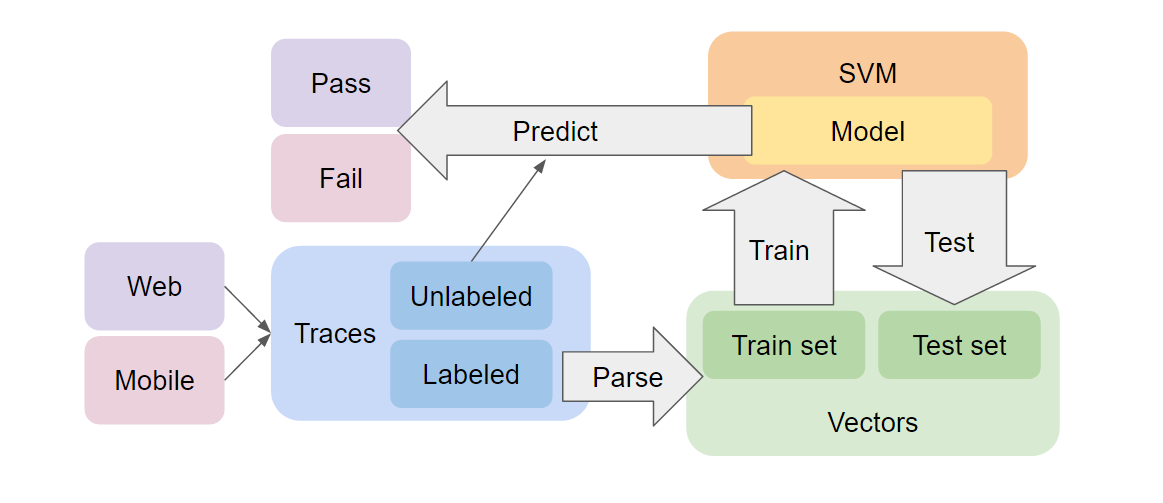
\includegraphics[width=0.8\textwidth]{EvaluateProcedure.png}
	\end{center}
	\caption{ The framework of testing. }
	\label{EvaluateProcedure}
\end{figure}

\clearpage


\chapter{Experiments}\label{ch:experiments}

We construct a tool WebTraceCollector for automatic web testing,
which can explore the website automaically and 
analyze the DOM tree of the current web page to find the next clickable element to click,
and propose a machine learning method to evaluate traces by SVM.
In order to use the tool and implement the evaluation, wee need a laptop and installing some tools.
The specification of the laptop we used is shown in Table[\ref{laptopSpec}],
and we need to install Windows, Python 3.4.3 and MySQL database.

\begin{table}[ht]
	\begin{center}
		\begin{tabular}{| l | l | }
			\hline
			Laptop & AUSU X450JN \\ \hline
			Operating System & Windows 10 (64bit) \\ \hline
			CPU & Intel(R) Core(TM) i5-4200 @2.8GHz \\ \hline
			RAM & 4GB \\ \hline
			Storage & 800G \\ \hline
		\end{tabular}
		\caption{ The specification of the laptop. }
		\label{laptopSpec}
	\end{center}
\end{table}

WebTraceCollector is constructed based on Python,
it control the browser by the selenium library and recognize the elements of the current page by the beautifulsoup library.
The automatic exploring mechanism highly depends on the page source downloaded from the current web page.
If the page source ot the constructed DOM tree can not match the current page correctly,
we can not find the correct clickable element and the testing may fail.
Thus, it is important to check how many web applications can download page soucre and construct DOM tree accurately.
In the experiment 1, we find 20 websites which is famous in taiwan.
We test those websites and generate traces automatically by WebTraceCollector.
Moreover, we want to check the ability of handling dynamic web pages.
We choose some common web pages with lots of input fields need to be inserted to test in the experiment 2.
In the experiment 3, we want to check the accuracy of the automatic prediction.
We generate some traces of certain applications and use those traces to train SVM model,
and we use this model to predict the traces of the applications.

\section{Trace collection}

In 20 popular applications\cite{popularWebs} that shown in Table \ref{popularWebs},
there are forums, news, community platforms, games and blogs.
We generate monkey traces by randomly click buttons and the length of traces is about 5.
The reason that we do not completely explore the whole website is most of the scale of websites are too big.
For example, a news website may have thousands of subpages and it may cost too much time to generate completely traces.
We just want to check the DOM tree is constructed correctly, 
so we make short traces to focus on checking the ability of clicking correct clickable elements.

The result of the experiments is shown in Table[].
There are 4 web applications that have serious problem on testing,
and most of web applications can be successfully explored with little defects.
There are two unkown fail happened, however it can work after restart the test.
The problems of the fail applications are 
too many iframes of advertising and API plugin in the webpages and buttons functions implemented by javascript.
The iframes become noise in the page source and make the DOM tree constructed incorrectly,
so WebTraceCollector may not find the correct clickable elements or only focus on the clickables in the advertising iframe.
On the other hand, the button functions in the web pages may implemented by javascript.
That means clickable elements may not be the style we thought, such as link tags or input-button tags,
it could be images, div tags or any tags if javascript bind the mouse listener on.
With the uncertain clickable elements, it is hard to find the correct clickable elements to explore the web and record the traces.
WebTraceCollector will click the wrong elements with nothing happens and stay at the same page until the trace is end.

\begin{table}[ht]
	\begin{center}
		\begin{tabular}{ | l | l | l | l | }
			\hline
			編號 & 網站名稱 & 網站類型 & URL \\ \hline
			1 & Facebook & Community platform & https://www.facebook.com/ \\ \hline
			2 & YouTube & Entertainment & https://www.youtube.com/ \\ \hline
			3 & Yahoo & Search engine & https://tw.yahoo.com/ \\ \hline
			4 & Google & Search engine & https://www.google.com.tw/ \\ \hline
			5 & 中時電子報 & News & http://www.chinatimes.com/ \\ \hline
			6 & 露天拍賣 & Commerce & http://www.ruten.com.tw/ \\ \hline
			7 & 聯合新聞網 & News & http://udn.com/news/index \\ \hline
			8 & 巴哈姆特 & Forum & http://www.gamer.com.tw/ \\ \hline
			9 & Mobile01 & Forum & http://www.mobile01.com/ \\ \hline
			10 & 蘋果日報 & News & http://www.appledaily.com.tw/ \\ \hline
			11 & 百度 & Search engine & https://www.baidu.com/ \\ \hline
			12 & 東森新聞雲 & News & http://www.ettoday.net/ \\ \hline
			13 & 卡提諾論壇 & Forum & http://ck101.com/ \\ \hline
			14 & 伊莉討論區 & Forum & http://www40.eyny.com/index.php \\ \hline
			15 & Hinet & Search engine & http://www.hinet.net/ \\ \hline
			16 & 微軟Live.com & Search engine & https://login.live.com/ \\ \hline
			17 & 痞客邦 & Blog & https://www.pixnet.net/ \\ \hline
			18 & PChome Online & Search engine & http://pchome.com.tw/ \\ \hline
			19 & 淘寶 & Commerce & https://world.taobao.com/ \\ \hline
			20 & Life生活網 & Blog & http://www.life.com.tw/ \\ \hline
			21 & 104人力銀行 & Survice & http://104.com.tw/ \\ \hline
			22 & 騰訊網  & Search Engine & http://www.qq.com/ \\ \hline
			23 & 新浪微博 & Community platform & http://www.weibo.com/login.php \\ \hline
			24 & 自由時報電子報 & News & http://www.ltn.com.tw/ \\ \hline
			25 & 維基百科 & Dictionary & https://www.wikipedia.org/ \\ \hline
		\end{tabular}
		\caption{ The 20 popular websites. }
		\label{popularWebs}
	\end{center}
\end{table}

\begin{table}[ht]
	\begin{center}
		\begin{tabular}{ | l | l | l | l | }
			\hline
			26 & 博客來 & Commerce & http://www.books.com.tw/ \\ \hline
			27 & 今日新聞網 & News & http://www.nownews.com/ \\ \hline
			28 & 商業周刊 & News & http://www.businessweekly.com.tw/ \\ \hline
			29 & 隨意窩Xuite & Blog & http://xuite.net/ \\ \hline
			30 & 1111人力銀行 & Survice & http://www.1111.com.tw/ \\ \hline
			31 & Flickr & Community platform & https://www.flickr.com/ \\ \hline
			32 & Blogger & Blog & http://www.blogger.com/ \\ \hline
			33 & 批踢踢實業坊 & Community platform & https://www.ptt.cc/index.html \\ \hline
			34 & FC2 & Survice & http://fc2.com/ \\ \hline
			35 & 卡卡洛普 & Survice & http://www.gamme.com.tw/ \\ \hline
			36 & PChome商店街 & Commerce & http://www.pcstore.com.tw/ \\ \hline
			37 & Giga Circle & Survice & http://tw.gigacircle.com/ \\ \hline
			38 & 鉅亨網 & News & http://www.cnyes.com/ \\ \hline
			39 & momo購物網 & Commerce & http://www.momoshop.com.tw/main/Main.jsp \\ \hline
			40 & 蕃薯藤 & Search engine & http://www.yam.com/ \\ \hline
			41 & OB嚴選 & Commerce & http://www.obdesign.com.tw/ \\ \hline
			42 & GOMAJI & Commerce & http://www.gomaji.com/Taipei \\ \hline
			43 & 愛評網 & Survice & http://www.ipeen.com.tw/ \\ \hline
			44 & 123KUBO酷播 & Entertainment & http://www.123kubo.com/ \\ \hline
			45 & 591租屋網 & Commerce & https://www.591.com.tw/ \\ \hline
			46 & TEEPR趣味新聞 & News & http://www.teepr.com/ \\ \hline
			47 & KKBOX & Entertainment & https://www.kkbox.com/tw/tc/index.html \\ \hline
			48 & msn台灣 & Search Engine & http://www.msn.com/zh-tw/ \\ \hline
			49 & 微軟 & Survice & https://www.microsoft.com/zh-tw/ \\ \hline
			50 & T客邦 & Blog & http://www.techbang.com/ \\ \hline
		\end{tabular}
	\end{center}
\end{table}

%針對20個網站做20個monkey traces的結果
%有些網站太複雜 iframe太多,太相似

\clearpage

\section{Dynamic webpages}

In order to test the ability of explore dynamic webpages,
we select some webpages that have lots of input fields and it need to insert correct values to pass through the web pages.
The selected webpages are shown in Table \ref{DynamicWebs}.
Most of the input fields in those web pages are names, years, emails and so on.
We can see that there are 4 web pages can be successfully passed through, but 3 web pages can not.
There are 3 reasons that can not pass through the dynamic web pages are the follows:
\\	1. The web pages have robot checking mechanism to prevent automatic exploring.
\\	2. The form of input fields are different to the examples in the database.
\\	3. The input fields are out of the range of examples we collecteed.
	
In reason 1, the robot checking like image recognition is developed to prevent people exploring the website automatically be computer.
It is too hard to find out the correct value by program,
and it is unreasonable if we can easily pass through those web pages.
If we want to test those websites,
the reasonable way is let the developers of the websites turn off the robot ckecking.

In reason 2, even though we have collect the examples of the input fields in the database, 
it is still a hard work to find out the correct form of the values.
For instance, we analyze the input field and find out the value should be a string of address.
But the type of input fields can be text, checkbox or selects, 
it is too hard to analyze user should insert the whole string of address or select each partens of area.

In reason 3, the web pages can have unlimited kinds of input fields.
Although we can add as more examples and rules in the database as we possible,
it is still impossible to handle all kinds of input fields by only few kinds of examples.
In future work, we can develop to find out the values by other method such as maching learning.

\begin{table}[ht]
	\begin{center}
		\begin{tabular}{ | l | l | }
			\hline
			URL & Result \\ \hline
			http://www.plurk.com/signup & Pass \\  \hline
			https://ups.moe.edu.tw/Personal\_Page/index.php & Pass \\  \hline
			https://applyweb.collegenet.com/account/new/create  & Pass \\  \hline
			https://apply.grad.ucsd.edu/signup  & Pass \\  \hline
			https://user.gamer.com.tw/regS1.phpt  & Fail \\  \hline
			http://panel.pixnet.cc/signup/step2  & Fail \\  \hline   
			https://apps.grad.uw.edu/applForAdmiss/newUserProfile.aspx?bhcp=1 & Fail \\  \hline 
		\end{tabular}
		\caption{ The dynamic webpages. }
		\label{DynamicWebs}
	\end{center}
\end{table}

%針對5個有inputs的網站做traces
%有的網站可以通過 有的只能一次(註冊) 有的偶爾可以(登入) 有的不行

\clearpage

\section{Prediction}

In this experiment, we focus on the ability of automated predicting passed traces and failed traces.
We select two web applications to use in our study and analysis their results.
The first web application is a small website about restraurant with simple buttons, 
and the second web application is a more complex website about APP store.
Before comparing the results of predicting traces between different applications,
we should collect the passed traces and failed traces from those web applications first.
Thus, we generate the random traces automatically by the tool WebTraceCollector introduced above
and select certain buttons and screens as the failed traits.

The traces with the specific buttons or screens will be labeled as failed traces and the other traces will be labeled as passed traces.
The detailed information of traces collected from the two web applications is shown in Table \ref{WebtracesProporiton} .
We can see that the percentage of failed traces is low.
The reason is that if the bugs are not occur at the main functionf of the applications,
there will be only a few traces triggering the bugs.

After collecting traces, the traces should be divided into training set for training SVM model and testing set.
We randomly devide the traces into two sets,
and repeat the experiments with different proportion of training set.
The result of prediction traces of application 1 is shown in Table \ref{PredictResult}.
Notice that the accuracy of prediction may not be better than just predicting every traces to pass,
because the number of failed trace is smaller than the number of passed trace.

Even though the prediction can not enhance the accuracy,
it still can help people finding failed traces.
The precision is the number of traces predicted failed that actually failed devided by the number of traces predicted as failed, 
which means the accuracy of predicting failed trace.
With the higher precision, it will be more convinced the traces predicted to be failed is actually failed.
If the precision is high enough, it can reduce human effort by predicting the failed traces with the convinced model.

The recall is the number of traces predicted failed that actually failed devided by the number of failed traces,
which means the ability of finding the failed traces in all traces.
With the higher recall, it will be more convinced that the system can find all the failed traces.
If the recall is high enough, it can reduce human effort by finding the failed traces with the convinced model.

We can obeserve that the accuracy of prediction in application 1 is about 0.65 ~ 0.75.
The average of precision is about 0.5 and the average of recall is about 0.45 but larger range.
From the result, we can say that the predictive model can find almost half of the failed traces in testing set,
and the half of the predicted traces are actually failed.

The result of prediction traces of application 2 is shown in Table \ref{PredictResult2}.
We can obeserve that the accuracy of prediction in application 1 is about 0.75 ~ 0.85.
The average of precision is about 0.5 and the average of recall is about 0.45 but larger range.
However, there are models that have very low precision and recall in some iterations.
It seems that sometimes SVM can not build a reliable model from training.
Because the web application 2 is more complex than application 1 
and the feature keywords is not precise enough to present the difference between passed traces and failed traces.
It will be hard to learn the predictive model of application 2.
The proportion of negative labels is another problem.
Because the amount of failed traces of application 2 is less than the failed traces of application 1,
The method of deviding traces into training set and testing set has a greater influence on learning model.
If we can not find the most important trace for training,
it will be difficult to learn the model and result in poor outcome.

Although the results of automated prediction shown in the above experiments is not good enough to replace all human effort,
it is still a feasible method for reducing the cost of web application testing.
In order to increase the accuracy of automated predicting,
the future work we need to do is to collect more keywords precisely and find other method of deviding traces into training set.
We can select the traces to trainging set depending on which trace can maximize the feature coverage or which trace has the least confident.
We can also use other machine learning algorithm, such as deep learning, to construct the predictice model.

\begin{table}[ht]
	\begin{center}
		\begin{tabular}{ | l | c | c | c | c | }%對同種類的網站 APP 和WEB 做traces
			\hline%測出其中有BUG
			Web Application & Total traces & Pass traces & Fail traces &  Negative Proportion \\ \hline
			Restraurant & 122 & 86 & 36 & 29.5\% \\ \hline
			APP Store & 94 & 84 & 10 & 10.63\% \\ \hline
		\end{tabular}
		\caption{ The number of passed traces and failed traces. }
		\label{WebtracesProporiton}
	\end{center}
\end{table}


\begin{table}[ht]
	\begin{center}
		\begin{tabular}{ | l | c | c | c | c | }
			\hline
			Application 1 & Training & Accuracy & Precision & Recall \\ \hline
			Repeat 1 & 0.4 & 0.7436 & 0.5  & 0.4  \\ \hline
			Repeat 2 & 0.4 & 0.75   & 0.64 & 0.5  \\ \hline
			Repeat 3 & 0.4 & 0.6486 & 0.5  & 0.46 \\ \hline
			Repeat 4 & 0.4 & 0.7333 & 0.53 & 0.69 \\ \hline
			Repeat 5 & 0.4 & 0.7209 & 0.63 & 0.46 \\ \hline
			Repeat 6 & 0.4 & 0.6667 & 0.45 & 0.45 \\ \hline
			Repeat 7 & 0.4 & 0.6154 & 0.35 & 0.6  \\ \hline
			Repeat 8 & 0.6 & 0.7272 & 0.5  & 0.5  \\ \hline
			Repeat 9 & 0.6 & 0.7307 & 0.5  & 0.43 \\ \hline
			Repeat 10& 0.6 & 0.6667 & 0.6  & 0.43 \\ \hline
			Repeat 11& 0.6 & 0.6087 & 0.43 & 0.38 \\ \hline
			Repeat 12& 0.6 & 0.7407 & 0.67 & 0.45 \\ \hline
			Repeat 13& 0.6 & 0.750  & 0.57 & 0.67 \\ \hline
			Repeat 14& 0.6 & 0.70   & 0.67 & 0.5  \\ \hline
		\end{tabular}
		\caption{ The prediction of Application 1. }
		\label{PredictResult}
	\end{center}
\end{table}

\begin{table}[ht]
	\begin{center}
		\begin{tabular}{ | l | c | c | c | c | }
			\hline
			Application 1 & Training & Accuracy & Precision & Recall \\ \hline
			Repeat 1 & 0.4 & 0.833  & 0.4  & 0.66  \\ \hline
			Repeat 2 & 0.4 & 0.891  & 1.0  & 0.33  \\ \hline
			Repeat 3 & 0.4 & 0.857  & 0.5  & 0.33  \\ \hline
			Repeat 4 & 0.4 & 0.920  & 1.0  & 0.33  \\ \hline
			Repeat 5 & 0.4 & 0.8787 & 0.5 & 0.25   \\ \hline
			Repeat 6 & 0.6 & 0.85   & 0.3  & 0.5   \\ \hline
			Repeat 7 & 0.6 & 0.88   & 0.4  & 1.0   \\ \hline
			Repeat 8 & 0.6 & 0.666  & 0.125& 0.5   \\ \hline
			Repeat 9 & 0.6 & 0.8    & 0.2  & 1.0   \\ \hline
			Repeat 10& 0.6 & 0.6363 & 0.1  & 1.0   \\ \hline
		\end{tabular}
		\caption{ The prediction of Application 2. }
		\label{PredictResult2}
	\end{center}
\end{table}

\chapter{Conclusion}\label{ch:conclusion}
\end{doublespace}

%\printbibliography

\clearpage\end{CJK*}
\end{document}
